\subsubsection{Missatges d'error del SDK}

\paragraph{}
En cas que alguna operació del SDK no acabi de la forma prevista, s'ensenya un error indicant que el problema ha recaigut a la banda de FamilySearch i s’indica el missatge d’error retornat des de l’organització.

Per exemple, en aquesta funcionalitat, és normal que certes persones retornades no existeixin realment a l'arbre. L'estil utilitzant per representar l'error és el mateix que pels errors de validació de formulari.

La imatge~\ref{fig:fsError} ensenya un d’aquests possibles missatges d’error.

\begin{figure}[h]
    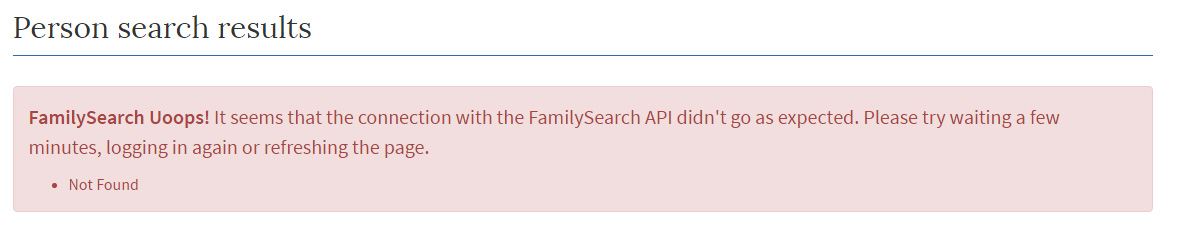
\includegraphics[width=\linewidth]{11/02_searchPersons/05_familySearchError}
    \centering
    \caption{Exemple de missatge d'error del SDK}\label{fig:fsError}
\end{figure}
